%************************************************
\chapter{Descripción de compresión JPEG con pérdida}\label{ch:jpeg_desc}
%************************************************

\section{Historia y Descripciones Breves de los Fundamentos Matemáticos}

La Teoría de Codificación es una sub-rama de la Teoría de la Información que
marcó el inicio del estudio formal de la compresión de datos. La Teoría de la
Información, nacida en 1948 con la publicación del artículo de Claude E.
Shannon ``A Mathematical Theory of Communication'' \cite{shannon}, gira
alrededor de los conceptos de \emph{densidad de información}, \emph{entropía de
información} y \emph{redundancia de información}.

La Codificación de Entropía son métodos de compresión sin pérdida de
información que no toman en cuenta el contenido. Los dos métodos más populares
actualmente son los Códigos de Huffman y la Codificación Aritmética.

Dos años después de la publicación de Shannon, David Huffman inventó lo que hoy
conocemos como Codificación Huffman \cite{Huffman}. Los Códigos de Huffman son
códigos de prefijos que minimizan la longitud de los códigos individuales. Se
mantienen hasta hoy como la técnica más aprovechada en algoritmos de compresión
sin pérdida.

Después de Huffman, el método más popular para reducir redundancia es la
Codificación Aritmética. Es un método más sofisticado que consigue mejores
resultados. Entre $5\%$ y $10\%$ según el estándar JPEG \cite{jpeg-spec}. La
especificación de la compresión JPEG incluye la capacidad de utilizar
codificación aritmética, pero en la práctica no tiende a ser usada. En
particular, las implementaciones de código abierto no podían usar legalmente
Codificación Aritmética ya que es una técnica altamente patentada
\cite{jpeg_patents}.

En 1974, Nasir Ahmed publicó un artículo describiendo su Transformada de Coseno
Discreta \emph{(DCT)}, por sus siglas en Inglés. La DCT es un caso particular
de la transformada de Fourier, restringida a los números reales.

La compresión JPEG como casi todos la usamos se basa en códigos de Huffman y en
la Transformada de Coseno Discreta.

% ============================================================
\section{Tipos de compresión}
% ============================================================

La compresión de datos puede ser \emph{con pérdida} o \emph{sin pérdida}. Una
compresión sin pérdida es una función biyectiva. El dominio de la función es el
espacio de datos que estamos interesados en comprimir. Los formatos de
compresión sin péridida funcionan identificando información redundante y
removiendo la redundancia, dejando la información intacta. La compresión con
pérdida hace esto también, pero también identifica información ``inecesaria''.
Dependiendo de la agresividad de la compresión, la pérdida de información puede
ser desde imperceptible a inaceptable.

El formato JPEG soporta varios tipos de compresión.

\begin{list}{}{} \item \emph{Baseline}

El tipo \emph{baseline} es el más popular y es el tipo de compresión en el que
se enfoca este trabajo. Por brevedad, a menos de que se especifique lo
contario, cuando el resto de este documento hable de compresión JPEG, estará
hablando del tipo \emph{baseline}. La compresión está basada en la Transformada
de Coseno Discreta para filtrar información innecesaria, y para reducir
redundancia puede utilizar Árboles de Huffman o Codificación Aritmética.

\item \emph{Progresivo}

El tipo \emph{progresivo} es similar a \emph{baseline}, pero se le agregan
propiedades deseables. La imagen se comprime en múltiples pasos, cada uno con
mayor detalle. Con el método \emph{progresivo}, se puede desplegar la imágen
sin que se tenga la totalidad de los datos en memoria.

La utilidad de este método es poder dibujar la imágen mientras se está
descargando de Internet. Cuando se está en un entorno con ancho de banda
limitado, o cuando se descarga una imágen muy grande, es de valor para el
usuario poder ver versiones de la imágen progresivamente más detalladas
mientras se descarga.

\item \emph{Sin pérdida}

La compresión sin pérdida fue agregada a JPEG ``por que tenían que'' y no hubo
un análisis riguroso para su diseño \cite{jpeg-spec}. Aunque la compresión JPEG
sin pérdida no es mala, formatos como PNG son altamente más populares y
efectivos. Mucho software simplemente no soporta JPEG con compresión sin
pérdida.

\item \emph{Compresión Jerárquica}

El modo jerárquico codifica la imágen en varias versiones, cada una a
diferentes resoluciones. Se guarda en una estructura ``piramidal''. La primera
imágen está comprimida a resolución completa, y cada imágen sucesiva se guarda
a la mitad de la resolución de la anterior. Esta pirámide se guarda en memoria
de imágen más pequeña a imágen más grande.

Este método es útil cuando la resolución de la imagen es muy grande, y la
aplicación no necesita o no es capaz de utilizar la imagen en su tamaño
completo.

\end{list}

% ============================================================
\section{Descripción de la Compresión \emph{Baseline} de JPEG}
% ============================================================

El codificador implementado en este trabajo es el \emph{Baseline JPEG}, al que
también se le refiere como \emph{DCT-Based Coding}, traducido aquí como
\emph{Codificación DCT}. Para el resto del documento, a menos que sea
necesario, se usará el término \emph{JPEG} para referirse a lo mismo que
\emph{Baseline JPEG}.

La codificación DCT divide a la imágen en bloques de $8\times8$ píxeles. Cada
bloque de $8\times8$ pasa por una serie de transformaciones y salen
secuencialmente como datos comprimidos.

El primer paso en el \emph{pipeline} es separar los componentes de la imágen.
Las dos maneras más comunes de representar imágenes en computadoras es
\verb+RGB+ o \verb+RGBA+: En ambos formatos, cada píxel ocupa 32 bits de
espacio, divididos en componentes de 8 bits. Cada componente corresponde a un
color o al valor de opacidad, comúnmente denominado \emph{alpha}. \verb+RGB+
corresponde al byte \verb+RRGGBBXX+, con \verb+RR+ representando rojo,
\verb+GG+ representando verde y \verb+BB+ representando azul. Aunque a veces
decimos que \verb+RGB+ es un formato de 24 bits, especificamos el byte
\verb+XX+ por convención, ya que siempre se utilizan 32 bits (4 bytes) para
representar RGB. \verb+RGBA+ es análogo a \verb+RGB+. Le corresponden los 4
bytes \verb+RRGGBBAA+, donde el último byte se usa para el valor \emph{alpha}.

\subsection{Endianness}

% Nota para edicion: DWORD es usado por intel & MS. No introducir nuestra propia pinche notación...

Cabe notar que diferentes plataformas tienen diferentes convenciones para
guardar colores en memoria. Windows espera que le mandemos píxeles en órden
\verb+BGRA+, ya que al inspeccionar la memoria se ve en el órden más familiar
de \verb+ARGB+ (Microsoft no ha dicho públicamente por qué reordenaron los
componentes de color pero no el de opacidad).

Este tema toca el concepto de \emph{endianness}, que es el término que usamos
para referirnos al orden de los bytes en una palabra de memoria. En
procesadores modernos, una palabra son 32 bits. 4 bytes, cada uno de 8 bits. La
mayoría de las instrucciones que se ejecutan toman palabras como parámetros, y
cuando nos importan los detalles de bajo nivel entonces debemos de entender la
diferencia entre arquitecturas \emph{little endian} y \emph{big endian}. Una
arquitectura \emph{Little endian} guarda los bytes de una palabra de izquierda
a derecha del menos significativo al más significativo. Es más claro usar el
ejemplo concreto de los colores representados en palabras de 32 bits. Un color
\verb+RGBA+ consiste de 4 bytes y en una máquina little endian se guarda en la
memoria de la computadora como \verb+ABGR+. En una máquina \emph{big endian},
se guarda de la misma manera en que lo escribirmos: \verb+RGBA+. En ambos tipos
de ordenamiento de memoria, su \emph{endianness} afecta sólamente al
ordenamiento de bytes dentro de palábras de máquina. No hay que confundirnos y
pensar que el efecto se extiende más allá de una palabra de 32 bits. Si tenemos
dos palabras \verb+U = abcd+ y \verb+V = efgh+ entonces \verb+UV+ se ve en
memoria como \verb+dcbahgfe+. Los bytes se voltean dentro de las palabras
individuales, pero las palabras siempre van de izquierda a derecha.
Procesadores ARM después de la versión 3 son \emph{bi-endian}; pueden
seleccionar su \emph{endianness} desde software.

En ensamblador con sintaxis de Intel o en el API de Windows, se utiliza
\verb+BYTE+ para denotar 8 bits, \verb+WORD+ para 16 bits, \verb+DWORD+ para 32
bits y \verb+QWORD+ para 64 bits. Esta convención viene de cuando los
procesadores eran de 16 bits, y no cambió ni en la transición a 32 bits en los
90's ni en la transición a 64 bits en los 00's

El codificador JPEG que escribimos asume que la máquina en la que se está
corriendo es \emph{little endian}.


\subsection{La DCT}

La transformada discreta de coseno, \emph{DCT} por sus siglas en Inglés, puede
representar $N$ puntos como una suma con pesos de funciones cosenoidales de
diferentes frecuencias. Es popular en compresión porque las señales que
comprimimos tienden a tener una representación con bajas frecuencias
predominantes. Por ejemplo, es más común una imagen de un cielo azul que ruido
blanco en todos los colores. Una imagen de un cielo azul tiene muy poca
variación, que al aplicar \emph{DCT} resulta en un peso alto para frecuencias
bajas y pesos más cercanos a cero para frecuencias más altas.

En JPEG, se divide la imagen en bloques de $8\times8$ y se utiliza una
\emph{DCT} de $8\times8$:

\begin{equation}\label{eq:dct}
F(u, v) = \frac{1}{4} C(u)C(v) \sum_{x=0}^{7}\sum_{y=0}^{7}
f(x,y)*\cos{\frac{(2x+1)u\pi}{16}}\cos{\frac{(2y+1)v\pi}{16}}
\end{equation}

donde \[C(u), C(v) = \begin{cases}
        \frac{1}{\sqrt{2}} & \quad \text{para } u,v = 0\\
        1                  & \quad \text{para } u,v \neq 0\\
\end{cases} \]
\begin{eqnarray*}
    f(u, v) \text{ es un punto del bloque de } 8\times8 \text{ de la imagen }\\
    F(u, v) \text{ es la DCT para el punto } u,v\\
\end{eqnarray*}

De la ecuación \ref{eq:dct} se puede derivar directamente un algoritmo para la
\emph{DCT}, visto más a detalle en el capítulo \ref{ch:implementacion}.

La función $F$ definida en \ref{eq:dct} es una función continua e invertible, y
su inversa es:

\begin{equation}\label{eq:idct}
f(x, y) = \frac{1}{4} \sum_{x=0}^{7}\sum_{y=0}^{7} C(u)C(v) F(u, v)*
\cos{\frac{(2x+1)u\pi}{16}}\cos{\frac{(2y+1)v\pi}{16}}
\end{equation}

Nótese entonces que en teoría podemos convertir los puntos de cada bloque de $8\times8$ a su forma en DCT y de regreso. La ventaja de tener cada bloque como coeficientes DCT es que su representación nos permite decidir \emph{qué información perder}.

\subsection{La vida de un bloque}\label{sub:vida}


JPEG trabaja dividiendo a la imagen en bloques cuadrados de 8 píxeles de ancho
y alto. Si el tamaño de la imagen no es un múltiplo de ocho, se redondea al
siguiente número que sí lo es y es el trabajo del decodificador ignorar los
píxeles sobrantes. Cada bloque es independiente de los demás y por lo tanto el
algoritmo es altamente paralelizable. Es una buena coincidencia que las
arquitecturas de GPU de hoy en día trabajan con grupos de 64 \emph{threads}.

Cada bloque pasa por varias etapas antes de ser escrito a memoria como bits
comprimidos de JPEG.


\subsection{YUV}\label{sub:yuv}

Cada bloque crudo de la imágen se convierte en tres nuevos bloques, cada uno
correspondiente a un componente del modelo de color \verb+YUV+, también
denominado \verb+YCbCr+

Un modelo de color es una manera abstracta de representar colores. \verb+RGB+
representa colores como combinaciones de tres colores primarios. \verb+YUV+ los
representa en tres componentes, uno para Luminancia y dos de Crominancia.

Luminancia, también llamado Luma o \verb+Y+, es la intensidad de la imagen. La
Crominancia, también llamada Chroma describe el color de la imagen y se
codifica con dos componentes \verb+U+ o \verb+Cb+ y \verb+V+ o \verb+Cr+, donde
$U = Azul - Luminancia$ y $V = Rojo - Luminancia$.

El modelo de color \verb+YUV+ se inventó con la invención de la televisión a
color. La luminancia no es otra cosa que la imagen en blanco y negro. La
transición al color se hizo gradualmente transmitiendo la información de la
misma manera que antes, pero usando dos nuevos canales, \verb+U+ y \verb+V+. De
esta manera, el nuevo formato era compatible con televisiones en blanco y
negro, que sólo necesitaban la información de uno de los canales.

\begin{figure}[hb]
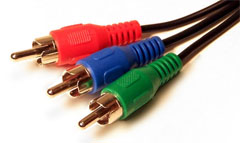
\includegraphics{yuv_cable}
    \caption{La siguiente generación no va a saber para que eran estos cables}
\end{figure}

Los cables RCA empezaron transmitiendo los tres componentes de \verb+YUV+. Más
tarde, cuando todos tenían color, se migró a usar un cable para \verb+YUV+,
llamado "video compuesto" y los otros dos para sonido estéreo.

\begin{figure}
    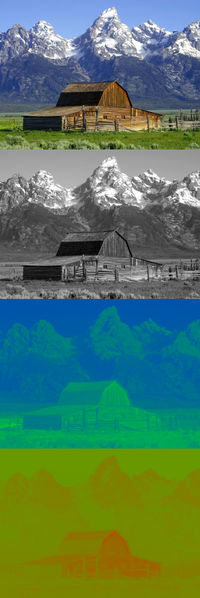
\includegraphics{yuv}
    \caption{Descomposición de una imagen a un canal de Luma y dos de Chroma}
\end{figure}

\verb+YUV+ tiene ventajas para comprimir imágenes. El sistema de visión humano
es mucho más sensible a cambios de intensidad en la imagen que a cambios de
color. Esto se aprovechaba en los días de la televisión analógica para utilizar
más ancho de banda en Luma que en Chroma, y el mismo principio se utiliza en
JPEG, cuya especificación incluye la opción de usar resoluciones más bajas para
los canales de chroma que el de luma. La implementación de \verb+tiny_jpeg+ usa
la misma resolución para los tres canales.

Los tres bloques correspondientes a \verb+Y+, \verb+U+, y \verb+V+ son escritos
al archivo en ese orden después de ser transformados independientemente.


\subsection{Aplicación de DCT y Cuantificación}\label{sub:vida_dct}

\begin{figure}[h]
    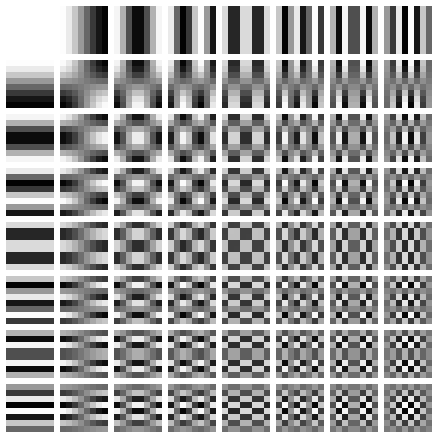
\includegraphics{DCT-8x8}
    \caption{Visualización de las funciones para el DCT de 8x8 usado en JPEG.
    Esquina superior izquierda: menor frecuencia. Inferior derecha: mayor
frecuencia.}
    \label{fig:dct}
\end{figure}



Al bloque se le aplica la Transformada Discreta de Coseno de $8\times8$. El
resultado son 64 coeficientes para las 64 funciones base. Como se muestra en la
figura \ref{fig:dct}, la frecuencia se incrementa hacia la derecha y abajo. Por
eso a partir de este momento se itera el bloque en un patrón de zig-zag
\ref{fig:zigzag}. Empezando en la esquina superior izquierda y acabando en la
inferior derecha.

\begin{figure}[h]
    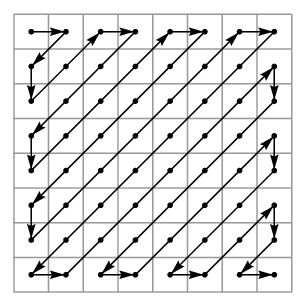
\includegraphics{zigzag}
    \caption{El patrón zig-zag con el que se itera por los bloques.}
    \label{fig:zigzag}
\end{figure}

En la descripción de la DCT se menciona que tener a cada bloque como
coeficientes DCT nos permite elegir educadamente qué información perder. En
principio, se pierde algo de información al aplicar la función DCT y luego su
inversa, sólo por el hecho de que estamos trabajando con una máquina con
precisión finita. Encima, el hecho de que JPEG especifica usar enteros de 10
bits o menos hace que se pierda un poco más información durante el proceso de
redondear valores de punto flotante. Aunque esos efectos de pérdida de
información no son negligibles, la principal manera en que se elige qué
información perder son las tablas de cuantificación.

Para cada codificador, usualmente elegido por heurísticas \emph{ a priori }, le
corresponde al menos dos tablas de cuantificación de 64 elementos. El propósito
de estas tablas es decidir cuanta información queremos perder para diferentes
coeficientes DCT. \emph{Cuantificación} es el proceso de convertir un conjunto
de valores a otro conjunto más pequeño. Para JPEG, usamos división entera para
cuantificar los elementos de cada bloque. El concepto se puede explicar con un
ejemplo:

Supongamos que tenemos el conjunto de valores $ \{ 1, 5, 103, 128, 242 \} $ que
queremos cuantificar usando división entera: Todos los elementos $e_i$ se
reducen a $ n_i \text{ tal que } e_i = n_i * c + r \text{ con } n \in ℕ \text{
y } c \text{ la constante de cuantificación }$. Para nuestro ejemplo, escogemos
$ c = 100 $. Con esta constante, el conjunto se cuantifica a $ \{ 0, 1, 2 \}$ .

\begin{eqnarray*}
    1 = 0 * 100 + 1 \\
    5 = 0 * 100 + 5 \\
    103 = 1 * 100 + 3 \\
    128 = 1 * 100 + 28. \\
    242 = 2 * 100 + 42.
\end{eqnarray*}

Se puede observar que mientras más grande sea la constante de cuantificación,
más elementos van a reducirse. También se puede ver que cuantificar con una
constante de $1$ resulta en el mismo conjunto de elementos. Es decir, \emph{ la constante 1 no resulta en pérdida de información.}

En JPEG, asociamos una constante de cuantificación a cada frecuencia de la DCT.
De esta manera es que se controla la \emph{pérdida} de información. Cuando el
usuario desea obtener la calidad máxima de imagen, se utilizan tablas de
cuantificación cuyas constantes son todas 1, en cuyo caso, la única pérdida de
información es la de redondeo y la de precisión de punto flotante.

En la práctica, se utiliza el hecho de que el sistema de visión humano es menos
sensible a cambios pequeños en frecuencias altas para escoger constantes
grandes para frecuencias altas y constantes pequeña para frecuencias bajas.
Sigue un ejemplo dado en \cite{jpeg-paper} para una tabla de cuantificación
típica:

\begin{equation}
    \begin{matrix}
        16 & 11 & 10 & 16 & 24  & 40  & 51  & 61 \\
        12 & 12 & 14 & 19 & 26  & 58  & 60  & 55 \\
        14 & 13 & 16 & 24 & 40  & 57  & 69  & 56 \\
        14 & 17 & 22 & 29 & 61  & 87  & 80  & 62 \\
        18 & 22 & 37 & 56 & 68  & 109 & 103 & 77 \\
        24 & 35 & 55 & 65 & 81  & 103 & 113 & 92 \\
        49 & 64 & 78 & 87 & 103 & 121 & 120 & 101 \\
        72 & 92 & 95 & 98 & 112 & 100 & 103 & 99
    \end{matrix}
    \label{fig:reference-table}
\end{equation}
\label{eq:cuantificacion}

Nótese que los valores crecen a la derecha y hacia abajo, hacia las frecuencias
altas, mientras que los valores mínimos se concentran en la esquina superior
izquierda en las frecuencias bajas (ver imágen \ref{fig:dct}).

Una manera de conseguir distintos niveles de calidad es dividir cada elemento
de la tabla de cuantificación por una constante. La tabla
\ref{eq:cuantificacion} se usa en la implementación de JPEG, con una constante
para controlar la calidad.

Aquí es donde la utilidad de los algoritmos genéticos entra en juego. Dado un
nivel de calidad deseado, es imposible encontrar una tabla de cuantificación
óptima para todas las imágenes. Una fotografía de un cielo azul puede
prescindir de frecuencias altas, mientras que un acercamiento a un suelo
arenoso perdería muchísima calidad. La estrategia para obtener tablas de
cuantificación ideales para imágenes individuales se explica en detalle en
\ref{ch:evolucion}


Después de la cuantificación, se codifica cada coeficiente como un entero de
longitud variable (\emph{VLI} por sus siglas en inglés).

El procedimiento \emph{VLI} convierte un número \verb+x+ en una tupla \verb+(n, x & (1 << n) - 1 )+
donde \verb+n+ es la longitud en bits necesaria para
representar \verb+x+ y el segundo término de la tupla es el valor restringido a
la precisión de \verb+n+ bits.

Un VLI es un tipo de datos de bajo nivel. Consiste de una longitud, que siempre
es de tamaño fijo, seguido de un número variable de bits que representan el
número.

Como ejemplo, digamos que queremos escribir el número 3. Se puede representar
en binario como \verb+11+, con dos bits. Sin embargo, en C, típicamente usamos
8, 16, 32 o 64 bits para representar números. Usando VLI, podemos escribir el
número 2 seguido de los dos bits que representan 3. Combinado con codificación
Huffman, esta técnica reduce aún más la representación de la información.

\subsection{Coeficientes AC y DC}\label{sub:acdc}

El primer coeficiente de cada bloque, denominado \emph{coeficiente DC}, se codifica con \emph{codificación delta}. Se mantiene una variable delta, inicializada en cero. Para cada bloque depués del primero, la variable delta guarda el valor del primer coeficiente. Cada bloque codifica su primer coeficiente como la diferencia entre su propio coeficiente y el coeficiente anterior. La razón para esto es que la variación entre coeficientes DC consecutivos tiende a ser pequeña. En los experimentos hechos para paralelizar el algoritmo evolutivo, se notó que la compresión delta contribuye con alrededor de $15\%$ de compresión extra, comparado con una versión que no usa compresión delta para el coeficiente DC.

Los otros 63 coeficientes son denominados \emph{coeficientes DC}. Se comprimen en tuplas de dos elementos. El segundo elemento es un coeficiente distinto de cero, el primer elemento representa el número coeficientes iguales a cero que le preceden.

% descripción breve de Huffman.

\subsection{Codificación Huffman}\label{sub:huffman}

El paso final en la vida de un bloque es utilizar \emph{codificación de
entropía}, que es el nombre que le damos a los algoritmos que codifican
información independientemente de las características de su medio. JPEG usa
\emph{prefix trees} en particular, y la gran mayoría de las implementaciones
JPEG usan Árboles de Huffman. La especificación proporciona una segunda
alternativa a Huffman: codificación aritmética, de la cual se dará un breve
resúmen al final de esta sección.

Los árboles de Huffman se enseñan en la Facultad de Ciencias para la carrera de
Ciencias de la Computación en el curso de Estructuras Discretas.

Dado una lista de símbolos, (el abecedario, por ejemplo), queremos que los
símbolos más usados tengan una representación más compacta que los símbolos
menos usados.

En el Español, la letra A es la más común y la K es la menos frecuente.
\cite{Espanol} La diferencia en frecuencias es de tres órdenes de magnitud.
Esto es un ejemplo de la Ley de Benford en acción \cite{Benford}

Los códigos de Huffman ordenan una lista de símbolos y le asigna a cada úno un
código respectivo de longitud creciente.

Para generar los códigos, se usa un Árbol de Huffman, que es un árbol binario
de prefijos. La figura \ref{fig:huffman} muestra un árbol de Huffman para el
enunciado en inglés \emph{this is an example of a huffman tree}.

\begin{figure}[h]
    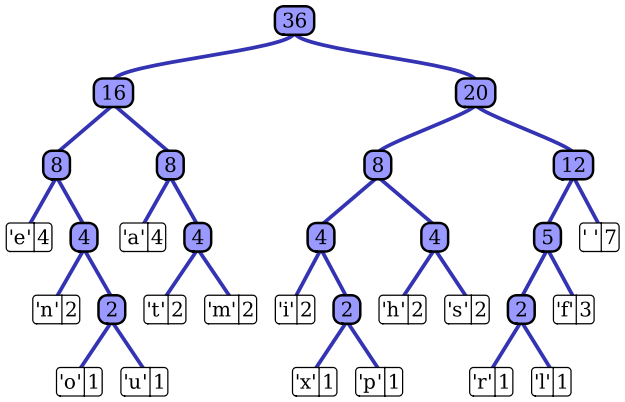
\includegraphics[width=1.0\textwidth]{Huffman}
    \caption{Ejemplo de un Árbol de Huffman}
    \label{fig:huffman}
\end{figure}

Los códigos se generan a partir del camino que se toma para llegar al símbolo
en el árbol. $0$ para rama izquierda, $1$ para rama derecha. En este ejemplo, a
la letra 'e' le corresponde el código \verb+000+ y a la letra 'a' \verb+001+.
Para estas dos letras se está usando 3 ($37.5\%$) de los 8 bits que se
necesitan comúnmente para representar letras en inglés.

El estándar proporciona un código de Huffman de referencia para las
implementaciones. Es el que comúnmente se usa y es el que nosotros usamos.
Depende del implementador hacer un código diferente para cada imagen, al costo
extra de tiempo de codificación y de complejidad de implementación.

La segunda opción que nos da la especificación es la \emph{Codificación
Aritmética}. No es popular, ya que hay muchas patentes relacionadas a la
técnica, pero para compresión es un método superior.

Aunque los Árboles de Huffman son óptimos para comprimir símbolos
separadamente, la Codificación Aritmética obtiene mejores resultados porque
codifica varios símbolos como coeficientes de polinomios. A cada símbolo le
corresponde un entero único correspondiente a la frecuencia en la que ocure, y
ese número se usa como el coeficiente. El grado del polinomio es la longitud
del mensaje.

\subsection{Resumen de la vida de un bloque}

Para recapitular. Lo que se hace en JPEG es (si es necesario) convertir la
imagen a \verb+YUV+, partirla en bloques de $8\times8$ para cada componente,
aplicar DCT a cada bloque y cuantificar, y finalmente, aplicar Codificación de
Huffman o Aritmética. Los bloques son escritos secuencialmente a disco en
formato \verb+YUV YUV YUV (...)+. Este trabajo se enfoca en usar heurísticas
para encontrar tablas de cuantificación cercanas a lo ideal.

%%% Local Variables:
%%% mode: latex
%%% ispell-local-dictionary: "espanol"
%%% TeX-engine: xelatex
%%% TeX-master: "../tesis"
%
